\documentclass[12pt,a4paper,oneside]{report}

\usepackage[utf8]{inputenc}
\usepackage[T1]{fontenc}
\usepackage{lmodern}
\usepackage{geometry}
\usepackage{microtype}
\usepackage{graphicx}
\usepackage{booktabs}
\usepackage{longtable}
\usepackage{array}
\usepackage{amsmath}
\usepackage{amssymb}
\usepackage{mathtools}
\usepackage{listings}
\usepackage{xcolor}
\usepackage{hyperref}

\geometry{
  left=30mm,
  right=25mm,
  top=25mm,
  bottom=25mm
}

\hypersetup{
  colorlinks=true,
  linkcolor=blue,
  citecolor=blue,
  urlcolor=blue,
  pdftitle={Hybrid Quantum-Classical Testbed for Operating System Scheduling},
  pdfauthor={TODO Student Name}
}

\graphicspath{{../results/}{../assets/image/}}

\lstdefinestyle{code}{
  basicstyle=\ttfamily\small,
  breaklines=true,
  frame=single,
  columns=fullflexible,
  showstringspaces=false,
  tabsize=2
}
\lstset{style=code}

\newcommand{\thesistitle}{Hybrid Quantum--Classical Testbed for Operating System Scheduling}
\newcommand{\studentname}{TODO Student Name}
\newcommand{\studentnumber}{TODO Student Number}
\newcommand{\supervisor}{TODO Supervisor Name}
\newcommand{\degree}{Bachelor Degree in TODO Degree Name}
\newcommand{\institution}{TODO University / Institute}
\newcommand{\department}{TODO Department}
\newcommand{\submissiondate}{TODO Month Year}
\newcommand{\todo}[1]{\textcolor{red}{[TODO: #1]}}

\begin{document}

\begin{titlepage}
  \centering
  \vspace*{20mm}
  {\Large \institution \par}
  \vspace{4mm}
  {\large \department \par}
  \vspace{22mm}
  {\Huge\bfseries \thesistitle \par}
  \vspace{18mm}
  {\Large Bachelor Thesis Report Base \par}
  \vfill
  \begin{tabular}{rl}
    Student: & \studentname \\
    Student number: & \studentnumber \\
    Supervisor: & \supervisor \\
    Degree: & \degree \\
  \end{tabular}
  \vfill
  {\large \submissiondate \par}
\end{titlepage}

\pagenumbering{roman}

\chapter*{Declaration}
\addcontentsline{toc}{chapter}{Declaration}
\todo{Replace this section with the official declaration required by your institution.}

I declare that this report is my own work and that all sources used have been
properly cited.

\chapter*{Acknowledgements}
\addcontentsline{toc}{chapter}{Acknowledgements}
\todo{Optional. Thank supervisors, colleagues, family, and anyone who supported the project.}

\chapter*{Abstract}
\addcontentsline{toc}{chapter}{Abstract}

Operating systems continuously decide how processes should share available CPU
resources. This project studies a restricted but representative scheduling
subproblem: assigning a set of processes or workload entities to a fixed number
of CPU cores while balancing total load. The work implements a research
prototype that maps process-to-core assignment to a Quadratic Unconstrained
Binary Optimization (QUBO) model and solves it with a hybrid
quantum--classical workflow based on the Quantum Approximate Optimization
Algorithm (QAOA).

The prototype includes a QUBO builder, a PennyLane-based QAOA solver, an exact
brute-force oracle for small instances, validation utilities, live process
tracing with \texttt{psutil}, adaptive clustering, iterative sub-QUBO
decomposition, visualizations, a Streamlit interface, and a TOML-driven
experiment runner. Small workloads are solved directly and compared against
brute force. Larger workloads are partitioned into sub-QUBOs that are solved
iteratively, with already assigned core loads propagated as bias terms.

Preliminary experiments show that the system can produce feasible assignments
for static and live workloads, match brute-force optima on several small
instances, and expose useful diagnostics such as optimality gap, load imbalance,
solver time, convergence curves, and feasibility status. The report concludes
that the prototype is suitable as an experimental testbed, while highlighting
limitations related to QAOA scalability, stochastic optimization, hardware
simulation, and the simplified scheduling model.

\textbf{Keywords:} operating system scheduling, QUBO, QAOA, hybrid
quantum--classical optimization, process scheduling, PennyLane.

\chapter*{Resumo}
\addcontentsline{toc}{chapter}{Resumo}
\todo{Translate the abstract to Portuguese if required by your institution.}

\tableofcontents
\listoffigures
\listoftables

\clearpage
\pagenumbering{arabic}

\chapter{Introduction}

\section{Context}

Modern operating systems must distribute runnable work across CPU cores while
reacting to changing process behavior, priorities, and resource demand. This is
traditionally handled with classical heuristics and carefully engineered kernel
policies. At the same time, quantum optimization methods have become an active
research direction for combinatorial problems that can be expressed as QUBO or
Ising models.

This thesis explores the intersection of these two areas through a research
prototype: a hybrid quantum--classical testbed for operating system scheduling.
The implemented project does not attempt to replace a production kernel
scheduler. Instead, it isolates a concrete scheduling decision, process-to-core
assignment, and studies how it can be modelled as a QUBO, solved with QAOA, and
validated against exact classical baselines for small cases.

\section{Problem Statement}

Given a set of workload entities with CPU weights and a fixed number of CPU
cores, the system must assign each entity to exactly one core. The main
optimization objective is load balancing: the final load of each core should be
as close as possible to the average load. In addition, the solution must respect
the one-hot assignment constraint, meaning that no process can be unassigned or
assigned to multiple cores.

The challenge is to express this assignment problem as a QUBO that can be
passed to a quantum-inspired or quantum-ready optimizer, while preserving enough
diagnostic information to evaluate feasibility, optimality, and scalability.

\section{Objectives}

The project has the following objectives:

\begin{enumerate}
  \item Formulate process-to-core scheduling as a QUBO model.
  \item Implement a QAOA-based solver using PennyLane.
  \item Validate small instances with an exact brute-force oracle.
  \item Provide a default pipeline for direct QUBO solving.
  \item Provide an iterative sub-QUBO pipeline for workloads that exceed a
  configurable qubit limit.
  \item Support both synthetic preset workloads and live process snapshots.
  \item Record experiment outputs and metrics in a reproducible format.
  \item Visualize matrices, convergence, probabilities, assignments, and
  iterative load evolution.
\end{enumerate}

\section{Main Contributions}

The main contributions of this work are:

\begin{itemize}
  \item A modular Python testbed for translating scheduling workloads into QUBO
  instances.
  \item A PennyLane QAOA solver supporting standard X mixing and an
  XY-style mixer designed to preserve one-hot feasibility.
  \item A validation layer comparing QAOA candidates against brute-force
  optima when the QUBO is small enough.
  \item A decomposition mechanism that partitions larger workloads into
  sub-QUBOs and propagates accumulated core-load bias between iterations.
  \item A live tracing and clustering path that converts real process snapshots
  into schedulable workload entities.
  \item A scenario runner and result format for repeated experiments.
\end{itemize}

\section{Document Structure}

Chapter~\ref{chap:background} introduces the relevant background. Chapter
~\ref{chap:formulation} defines the scheduling problem and QUBO model. Chapter
~\ref{chap:implementation} presents the system design and implementation.
Chapter~\ref{chap:methodology} describes the evaluation methodology. Chapter
~\ref{chap:results} reports preliminary results. Chapter~\ref{chap:discussion}
discusses findings and limitations. Chapter~\ref{chap:conclusion} concludes the
report and lists future work.

\chapter{Background}
\label{chap:background}

\section{Operating System Scheduling}

CPU scheduling decides which runnable process or thread should execute on each
processor core. Practical schedulers consider fairness, latency, throughput,
priority, affinity, cache locality, and real-time constraints. This project
focuses on a simplified scheduling subproblem: assigning already observed
workload entities to cores according to CPU demand. The model ignores many
kernel-level details, but it provides a controlled optimization target that can
be mapped to a QUBO. Standard operating-system scheduling concepts are covered
in texts such as \cite{silberschatz}.

\section{QUBO Models}

A QUBO problem minimizes a quadratic function over binary variables:

\begin{equation}
  \min_{x \in \{0,1\}^n} x^\top Q x ,
\end{equation}

where \(Q \in \mathbb{R}^{n \times n}\) is a matrix encoding linear and
quadratic terms. QUBO is useful because many combinatorial constraints can be
converted into penalty terms and incorporated into the objective
\cite{lucas2014ising,glover2018qubo}.

\section{Ising Hamiltonians}

QUBO variables can be mapped to Ising spin variables and then to quantum
operators. The common transformation is:

\begin{equation}
  x_i = \frac{1 - z_i}{2},
\end{equation}

where \(x_i \in \{0,1\}\) and \(z_i \in \{-1,1\}\). In the implemented solver,
the QUBO matrix is converted to a PennyLane Hamiltonian formed from Pauli-Z and
Pauli-Z pair terms.

\section{QAOA}

The Quantum Approximate Optimization Algorithm was introduced as a variational
method for approximate combinatorial optimization \cite{farhi2014qaoa}. It
alternates between a cost Hamiltonian and a mixer Hamiltonian. For \(p\) layers,
the parameterized state can be written as:

\begin{equation}
  \left|\psi(\boldsymbol{\gamma}, \boldsymbol{\beta})\right\rangle =
  \prod_{\ell=1}^{p}
  e^{-i \beta_\ell H_M}
  e^{-i \gamma_\ell H_C}
  \left|\psi_0\right\rangle .
\end{equation}

A classical optimizer updates the parameters
\(\boldsymbol{\gamma}, \boldsymbol{\beta}\) to minimize the expected cost.
This project uses Adam optimization through PennyLane and records the
convergence curve at each optimization step.

\section{Constraint-Preserving Mixers}

The project supports two mixer modes:

\begin{itemize}
  \item The X mixer prepares a uniform superposition over all bitstrings. This
  includes infeasible assignments.
  \item The XY-style mixer starts from a valid one-hot assignment and applies
  pairwise \(XX + YY\) interactions between core variables for the same
  process. The design goal is to move amplitude between valid core choices
  without leaving the one-hot subspace.
\end{itemize}

The implementation treats the XY mixer as a research feature and does not claim
hardware-level superiority. It is mainly useful for studying feasibility and
search behavior in this scheduling formulation.

\chapter{Problem Formulation}
\label{chap:formulation}

\section{Workload Model}

Let \(N\) be the number of workload entities and \(K\) the number of cores. Each
entity \(i\) has CPU weight \(w_i\). In preset workloads, these weights are
provided manually. In live mode, they are obtained from a process snapshot and
normalized relative to total logical CPU capacity.

The decision variable is:

\begin{equation}
  x_{i,k} =
  \begin{cases}
    1, & \text{if entity } i \text{ is assigned to core } k,\\
    0, & \text{otherwise.}
  \end{cases}
\end{equation}

The number of binary variables is therefore:

\begin{equation}
  n = N K .
\end{equation}

\section{Assignment Constraint}

Each entity must be assigned to exactly one core:

\begin{equation}
  \sum_{k=1}^{K} x_{i,k} = 1
  \quad \forall i \in \{1,\dots,N\}.
\end{equation}

The QUBO encodes this as a quadratic penalty:

\begin{equation}
  P \sum_{i=1}^{N} \left(\sum_{k=1}^{K} x_{i,k} - 1\right)^2 ,
\end{equation}

where \(P\) is the penalty weight.

\section{Load-Balancing Objective}

Let \(\phi_k\) represent load already fixed on core \(k\), for example from
real-time processes or from previous sub-QUBOs in the iterative pipeline. The
load of core \(k\) is:

\begin{equation}
  L_k = \phi_k + \sum_{i=1}^{N} w_i x_{i,k}.
\end{equation}

The target average load is:

\begin{equation}
  L_{\text{avg}} = \frac{\sum_{i=1}^{N} w_i + \sum_{k=1}^{K}\phi_k}{K}.
\end{equation}

The balancing term minimizes deviation from the average:

\begin{equation}
  \sum_{k=1}^{K} \left(L_k - L_{\text{avg}}\right)^2 .
\end{equation}

\section{Complete QUBO Objective}

The full objective used by the builder is:

\begin{equation}
  \min_x
  \sum_{k=1}^{K}
  \left(
    \phi_k + \sum_{i=1}^{N} w_i x_{i,k} - L_{\text{avg}}
  \right)^2
  +
  P \sum_{i=1}^{N}
  \left(\sum_{k=1}^{K} x_{i,k} - 1\right)^2 .
  \label{eq:qubo-objective}
\end{equation}

After expanding Equation~\ref{eq:qubo-objective} and dropping constants, the
implementation fills the QUBO matrix using the following coefficients:

\begin{align}
  Q_{(i,k),(i,k)}
  &= w_i^2 + 2w_i\phi_k - 2L_{\text{avg}}w_i - P, \\
  Q_{(i,k),(j,k)}
  &= w_i w_j
  \quad \text{for } i \neq j, \\
  Q_{(i,k),(i,l)}
  &= P
  \quad \text{for } k \neq l.
\end{align}

The energy of a candidate bitstring is computed as:

\begin{equation}
  E(x) = x^\top Q x .
\end{equation}

\section{Feasibility and Decoding}

A bitstring is decoded by mapping each active variable \(x_{i,k}=1\) to an
assignment \(i \mapsto k\). A solution is feasible if every entity appears
exactly once and every decoded value is a valid core identifier. This
feasibility check is used by both the QAOA solver and the brute-force validator.

\chapter{System Design and Implementation}
\label{chap:implementation}

\section{Architecture Overview}

The repository is organized as a modular runtime, with data contracts shared
between builders, solvers, pipelines, tracers, and visualizers. The main
orchestration API is \texttt{SchedulingEngine.run\_job(...)}.

\begin{lstlisting}[caption={High-level scheduling flow.}]
SystemSnapshot or preset weights
        |
        v
Workload
        |
        v
CoreAssignmentBuilder -> QUBOInstance
        |
        +--> PennylaneSolver  -> QAOA candidate
        |
        +--> BruteForceSolver -> exact reference for small QUBOs
        |
        v
SolverValidator -> feasibility, optimality, optimality gap
\end{lstlisting}

When the number of variables exceeds the configured qubit limit, the engine
uses an iterative decomposition flow:

\begin{lstlisting}[caption={Iterative sub-QUBO flow.}]
Global QUBO
  -> partition workload into groups
  -> extract sub-QUBO
  -> solve sub-QUBO with QAOA
  -> update assignments
  -> update phi core-load vector
  -> repeat
\end{lstlisting}

\section{Data Contracts}

The file \texttt{src/data\_contracts.py} defines the shared objects used across
the prototype. The most important contracts are:

\begin{itemize}
  \item \texttt{ProcessInfo}: traced or preset process metadata.
  \item \texttt{SystemSnapshot}: process list plus core and memory metadata.
  \item \texttt{Workload} and \texttt{WorkloadEntity}: scheduling abstraction
  consumed by the QUBO builder.
  \item \texttt{QUBOInstance}: Q matrix and variable metadata.
  \item \texttt{SolverResult}: bitstring, decoded assignments, energy,
  feasibility, probabilities, backend, and convergence curve.
  \item \texttt{SchedulingOutput}: direct/default pipeline output.
  \item \texttt{IterativeSchedulingOutput}: decomposed workload output,
  including final assignments and phi history.
\end{itemize}

\section{QUBO Builder}

The main builder is \texttt{CoreAssignmentBuilder}. It receives a
\texttt{Workload} and produces a \texttt{QUBOInstance}. For \(N\) entities and
\(K\) cores, it creates \(N K\) variables. The \texttt{variable\_map} field maps
each flat variable index to the corresponding \((\text{entity\_id},
\text{core\_id})\) pair.

The builder encodes the load-balancing objective and the one-hot assignment
penalty. It also supports fixed-load bias through \(\phi\), which is required by
the iterative pipeline.

\section{QAOA Solver}

The \texttt{PennylaneSolver} converts the QUBO matrix into an Ising Hamiltonian,
builds a QAOA circuit, optimizes parameters with Adam, and then ranks measured
probabilities to select a candidate bitstring. The solver attempts to use
\texttt{lightning.gpu}; if the GPU backend fails, it retries with
\texttt{lightning.qubit}. PennyLane provides the circuit construction,
automatic differentiation, and simulator backend interface used by this solver
\cite{pennylane}.

The configurable QAOA parameters are:

\begin{itemize}
  \item number of layers \(p\);
  \item number of optimizer steps;
  \item learning rate;
  \item number of ranked bitstrings inspected;
  \item mixer type, either \texttt{x} or \texttt{xy};
  \item initial \(\gamma\) and \(\beta\) values.
\end{itemize}

\section{Brute-Force Oracle and Validation}

For small QUBOs, \texttt{BruteForceSolver} enumerates bitstrings and returns the
minimum feasible solution. The current size guard avoids brute-force solving
above 22 variables. \texttt{SolverValidator} compares QAOA output against this
oracle and reports candidate energy, global energy, decoded assignments,
feasibility errors, and optimality status.

The project reports optimality gap as:

\begin{equation}
  \text{gap} =
  \frac{E_{\text{candidate}} - E_{\text{feasible optimum}}}
  {\left|E_{\text{reference}} - E_{\text{feasible optimum}}\right| +
  \varepsilon}.
\end{equation}

An optimality gap of zero means that the candidate matched the feasible
brute-force optimum.

\section{Default Pipeline}

The default pipeline is used when \(N K \leq \texttt{qubit\_max}\). It builds
the complete QUBO, solves it with QAOA, and validates the candidate directly.
This path is most useful for correctness checks and small controlled
experiments.

\section{Iterative Pipeline}

The iterative pipeline is used when the workload exceeds the configured qubit
limit. It first builds a global QUBO, partitions entities into groups, extracts
sub-QUBOs, and solves them one at a time. After each feasible sub-QUBO result,
the final assignment map and \(\phi\) vector are updated.

Bias propagation is applied by adding accumulated load to the diagonal terms:

\begin{equation}
  Q_{\text{diag}} \leftarrow Q_{\text{diag}} + 2 w_i \phi_k .
\end{equation}

If a sub-QUBO returns no feasible assignment, the pipeline raises
\texttt{InfeasibleSubQUBOError} before updating global state. This prevents a
fallback infeasible bitstring from contaminating later sub-QUBO solves.

\section{Live Tracing and Clustering}

Live process tracing is implemented with \texttt{psutil}. The tracer records
PID, command, current core, CPU weight, resident memory, priority, estimated I/O
wait ratio, and priority class. CPU weights are normalized to total logical CPU
capacity.

For larger live snapshots, \texttt{AdaptiveCluster} groups processes into
bundles. The current approach separates real-time priority processes from normal
processes, computes effective CPU demand, builds a feature matrix from CPU and
memory, constructs an RBF affinity matrix, applies spectral clustering, falls
back to KMeans when needed, and splits bundles that are too heterogeneous or
heavy.

\section{Visualization and User Interface}

The project includes Matplotlib visualizations for:

\begin{itemize}
  \item QUBO matrix heatmaps;
  \item energy landscapes;
  \item QAOA convergence curves;
  \item top probability bitstrings;
  \item final load balance;
  \item phi evolution across sub-QUBOs.
\end{itemize}

The Streamlit interface in \texttt{src/app.py} exposes single runs and sweeps.
The command-line interface in \texttt{src/main.py} provides a simple
experiment entry point.

\section{Experiment Runner}

Experiments are defined as TOML scenario files under
\texttt{src/experiments/scenarios}. The runner resolves QAOA, QUBO, tracer, and
decomposition configuration, executes selected scenarios, and writes both JSON
and readable text outputs under \texttt{src/experiments/results}. The stored
metrics include pipeline type, number of entities, number of variables,
feasibility, optimality, optimality gap, load imbalance, solve time, and final
assignments.

\chapter{Experimental Methodology}
\label{chap:methodology}

\section{Research Questions}

The evaluation is organized around the following research questions:

\begin{enumerate}
  \item Can the QUBO builder encode the process-to-core assignment problem
  correctly?
  \item Does the QAOA solver return feasible schedules on small static
  workloads?
  \item How often does QAOA match the brute-force feasible optimum on small
  instances?
  \item Does the XY-style mixer improve feasibility behavior compared with the
  standard X mixer?
  \item Can iterative decomposition preserve feasibility while reducing
  subproblem size?
  \item Can live process snapshots be converted into schedulable workloads and
  solved by the same pipeline?
\end{enumerate}

\section{Implementation Environment}

\begin{table}[h]
  \centering
  \caption{Software environment used by the prototype.}
  \label{tab:software-environment}
  \begin{tabular}{ll}
    \toprule
    Component & Version / role \\
    \midrule
    Python & 3.12 or newer \\
    Dependency manager & \texttt{uv} \\
    Quantum framework & PennyLane \\
    Quantum backend & \texttt{lightning.gpu}, fallback \texttt{lightning.qubit} \\
    Classical libraries & NumPy, scikit-learn, psutil \\
    User interface & Streamlit \\
    Visualization & Matplotlib \\
    Test framework & \texttt{unittest} \\
    \bottomrule
  \end{tabular}
\end{table}

\todo{Add the exact machine used for final experiments: CPU, GPU, RAM, operating
system, Python version, and whether QAOA used GPU or CPU simulation.}

\section{Scenario Tiers}

The experiment scenarios are grouped by tier and category. Table
~\ref{tab:scenario-tiers} summarizes the intended role of each tier.

\begin{table}[h]
  \centering
  \caption{Experiment scenario tiers.}
  \label{tab:scenario-tiers}
  \begin{tabular}{lll}
    \toprule
    Tier & Category & Purpose \\
    \midrule
    T1 & smoke & Minimal direct pipeline sanity checks \\
    T2 & correctness & Feasibility, optimality gap, mixer diagnostics \\
    T3 & decomposition & Forced and heuristic sub-QUBO decomposition \\
    T4 & scaling & Repeated medium-size and generated workloads \\
    T5 & live & Live process tracing and clustered workloads \\
    \bottomrule
  \end{tabular}
\end{table}

\section{Metrics}

The main metrics are:

\begin{itemize}
  \item \textbf{Feasibility}: whether each entity is assigned to exactly one
  core.
  \item \textbf{Optimality}: whether the candidate matches the feasible
  brute-force optimum when brute force is available.
  \item \textbf{Optimality gap}: normalized difference between candidate energy
  and feasible optimum.
  \item \textbf{Solve time}: time spent by the solver, in milliseconds.
  \item \textbf{Load imbalance}: difference between maximum and minimum final
  core load.
  \item \textbf{Max probability}: largest probability in the final QAOA output
  distribution.
  \item \textbf{Sub-QUBO feasibility}: fraction of iterative subproblems that
  produce feasible assignments.
\end{itemize}

\section{Unit Tests}

The test suite verifies the QUBO builder and brute-force oracle. Builder tests
check that variable counts, matrix shape, variable maps, metadata, coefficients,
and one-hot decoding behave as expected. Brute-force tests verify that the
oracle returns feasible assignments, computes energy consistently, finds the
minimum feasible energy, and refuses QUBOs that exceed its size guard.

\section{Reproducibility Procedure}

The following commands install dependencies, run tests, and execute scenarios:

\begin{lstlisting}[caption={Reproducibility commands.}]
make install
make all-tests
python3 src/experiments/scenario_runner.py --list
python3 src/experiments/scenario_runner.py --all
\end{lstlisting}

\todo{For the final report, record the exact command used for the final
experiment campaign and commit hash.}

\chapter{Results}
\label{chap:results}

\section{Preliminary Experiment Summary}

Table~\ref{tab:preliminary-results} provides a compact snapshot of preliminary
results already present in the repository. These values should be replaced by a
fresh final run before submission.

\begin{longtable}{p{24mm}p{19mm}rrrrp{18mm}p{18mm}p{20mm}}
  \caption{Preliminary results from current \texttt{latest\_result.json} files.}
  \label{tab:preliminary-results}\\
  \toprule
  Scenario & Pipeline & \(N\) & \(K\) & Vars. & Sub-QUBOs & Feasible & Optimal & Time (ms) \\
  \midrule
  \endfirsthead
  \toprule
  Scenario & Pipeline & \(N\) & \(K\) & Vars. & Sub-QUBOs & Feasible & Optimal & Time (ms) \\
  \midrule
  \endhead
  T1.1 minimal direct & default & 2 & 2 & 4 & -- & true & true & 668 \\
  T1.2 three-process direct & default & 3 & 2 & 6 & -- & true & true & 425 \\
  T1.3 qubit boundary & default & 4 & 2 & 8 & -- & true & true & 570 \\
  T2.3 one-hot feasibility & default & 4 & 2 & 8 & -- & true & true & 604 \\
  T2.4 X mixer stress & default & 4 & 2 & 8 & -- & true & true & 697 \\
  T2.5 three-core direct & default & 4 & 3 & 12 & -- & true & true & 1421 \\
  T3.1 forced decomposition & iterative & 4 & 2 & 8 & 2 & true & true & 841 \\
  T3.3 coupling descending & iterative & 6 & 2 & 12 & 2 & true & false & 1069 \\
  T3.4 multi-sub-QUBO stress & iterative & 8 & 2 & 16 & 3 & true & true & 1491 \\
  T3.5 three-core iterative & iterative & 5 & 3 & 15 & 2 & true & true & 1524 \\
  T4.1 medium direct repeated & default & 6 & 2 & 12 & -- & true & true & 3360 \\
  T4.2 medium iterative repeated & iterative & 6 & 2 & 12 & 2 & true & true & 3004 \\
  T4.3 generated larger iterative & iterative & 10 & 2 & 20 & 4 & true & true & 2936 \\
  T5.1 live trace small core count & iterative & 17 & 2 & 34 & 5 & true & n/a & 2175 \\
  T5.2 live trace realistic load & iterative & 32 & 4 & 128 & 16 & true & n/a & 38732 \\
  \bottomrule
\end{longtable}

\todo{Regenerate this table from one final experiment campaign. Include
confidence intervals or repeated-run statistics where possible.}

\section{Optimality Gap}

On small direct instances where brute force is available, several current
scenarios report an optimality gap of zero. This means the QAOA-selected
candidate matched the feasible brute-force optimum for those workloads. The
coupling-descending decomposition scenario currently reports a very small but
non-zero gap, indicating a feasible but not globally optimal assembled
assignment.

\section{Feasibility}

The current scenarios report feasible final assignments across both default and
iterative pipelines. This is important because a low QUBO energy alone is not
sufficient if the decoded bitstring violates the one-hot assignment constraint.
The explicit feasibility checks and the iterative infeasible-sub-QUBO guard are
therefore central to the reliability of the prototype.

\section{Load Balance}

Iterative outputs include \(\phi\) histories and final load imbalance. In
several static decomposition scenarios, the final imbalance is zero or close to
floating-point precision. Live scenarios also produce feasible assignments, but
their optimality is not reported when brute force is skipped due to QUBO size.

\section{Visual Outputs}

\begin{figure}[h]
  \centering
  \IfFileExists{../results/iterative_run.png}{
    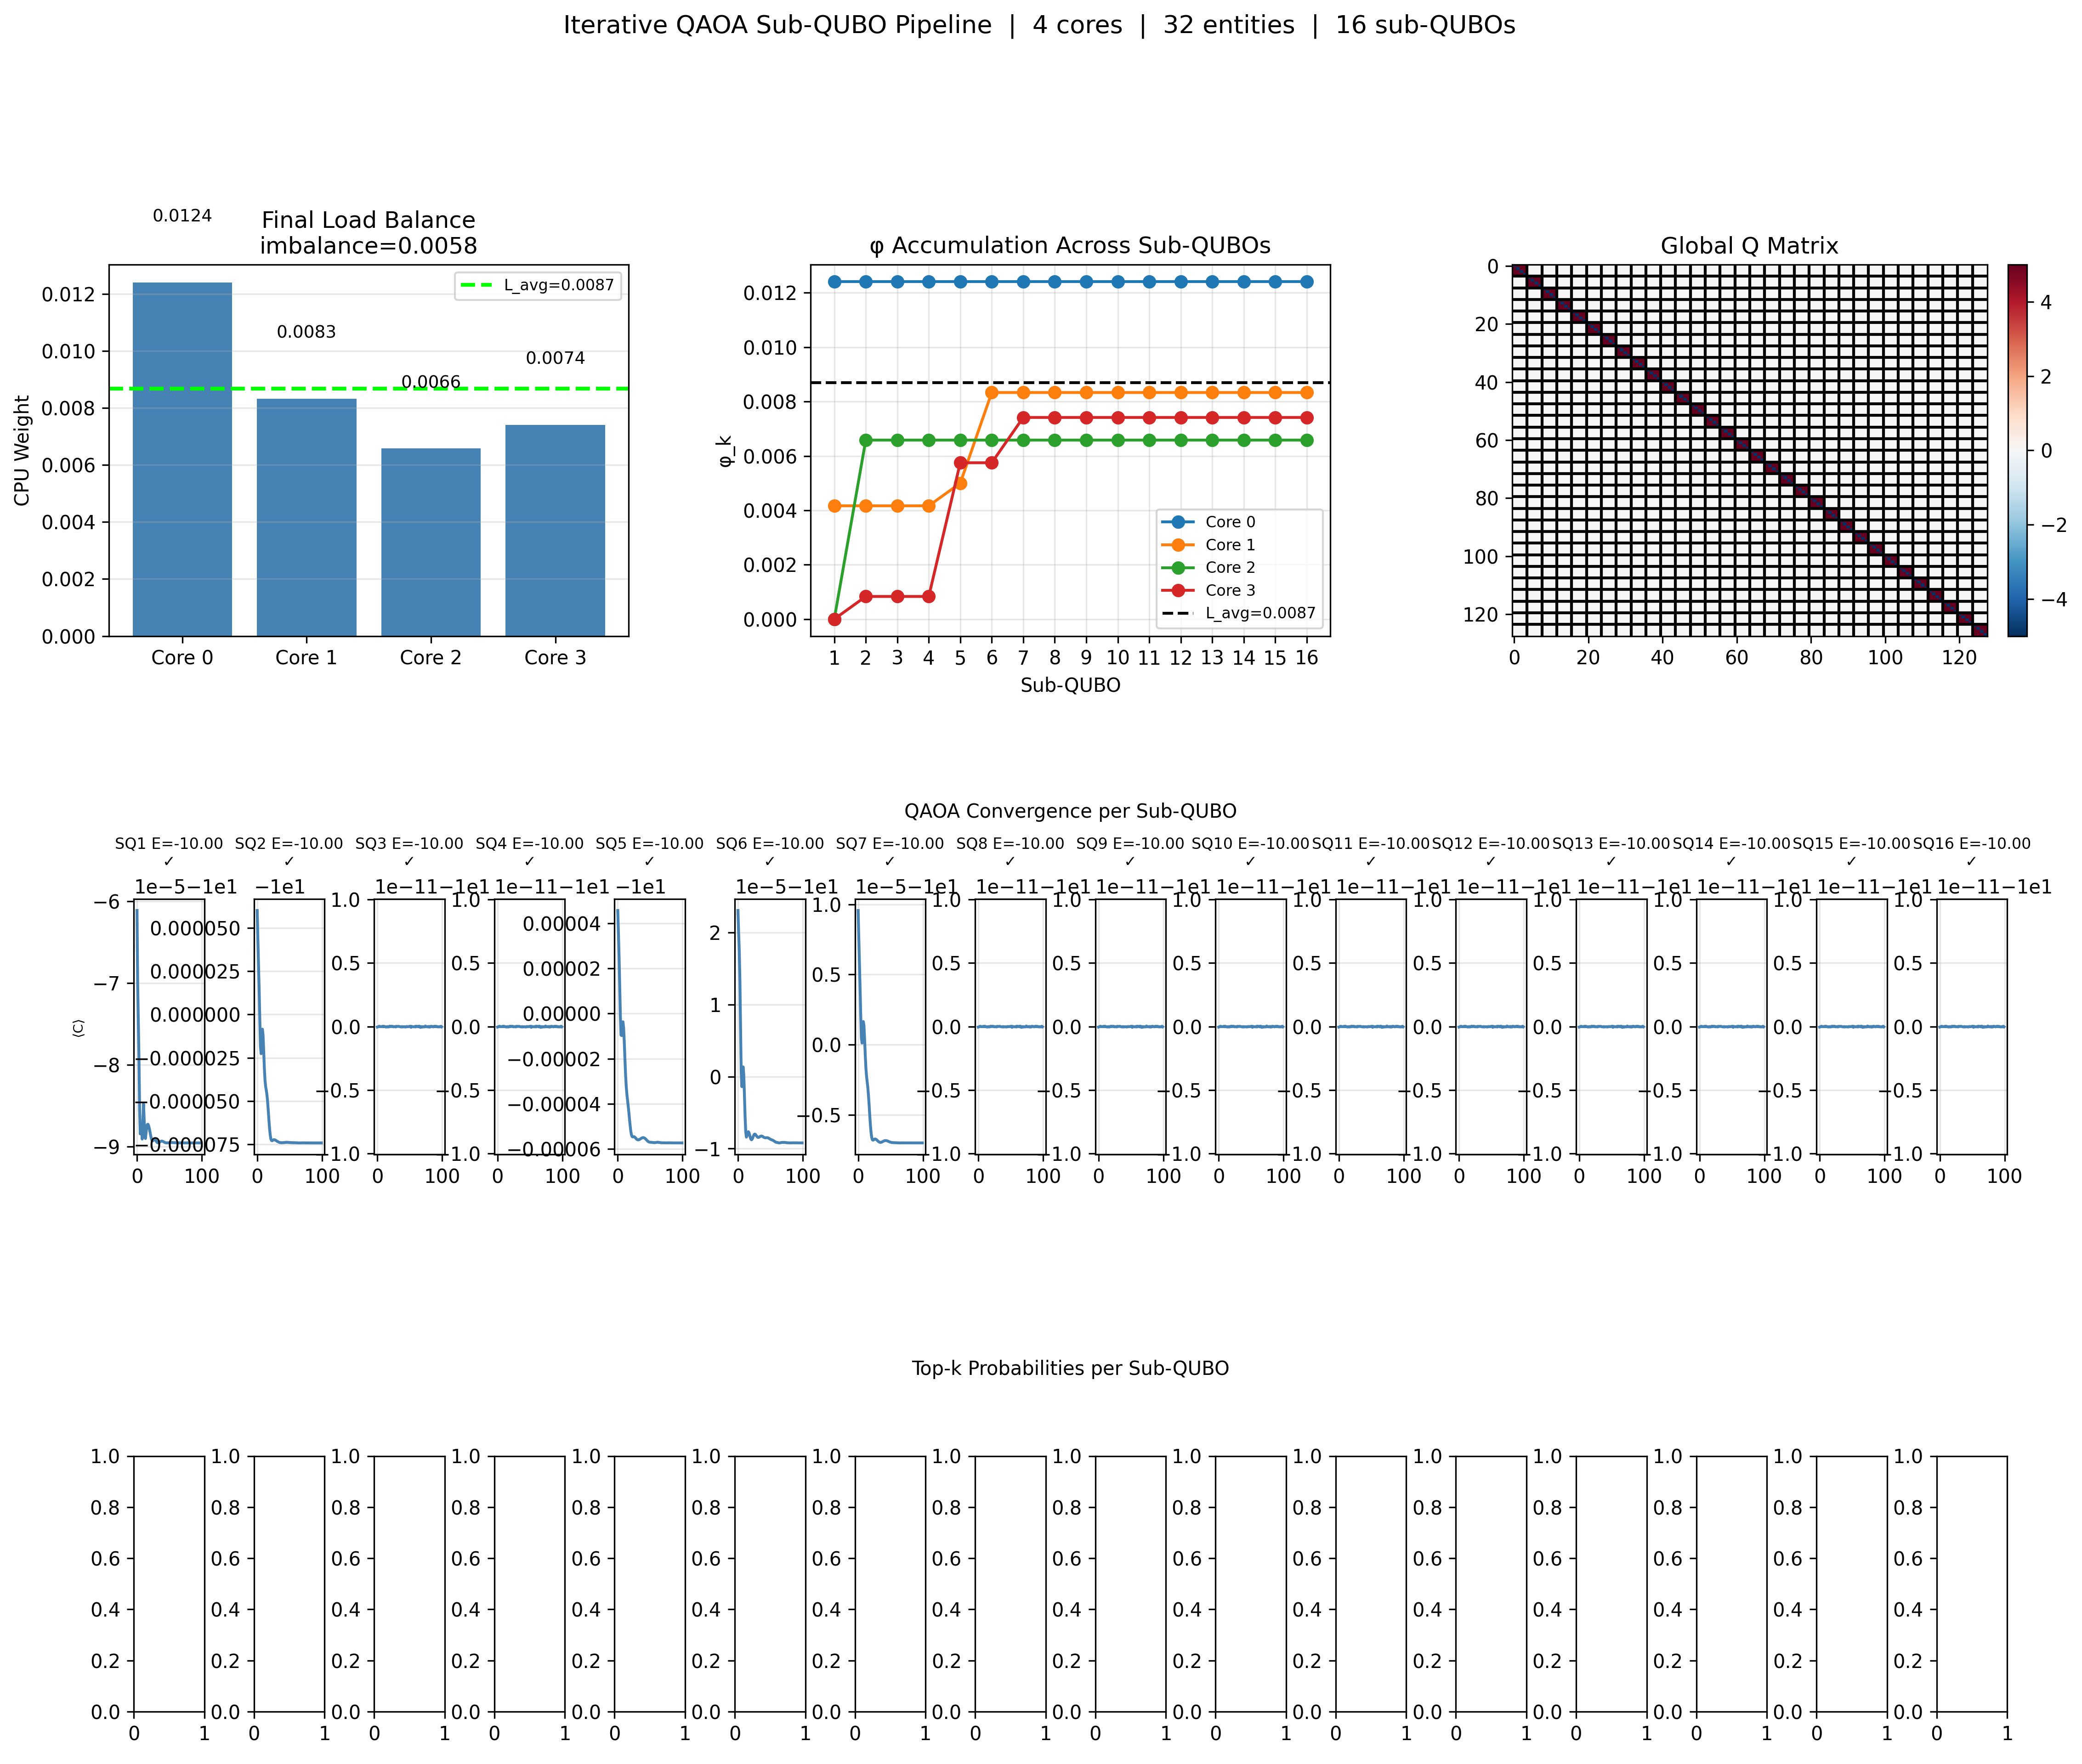
\includegraphics[width=0.9\textwidth]{../results/iterative_run.png}
  }{
    \fbox{\parbox{0.85\textwidth}{\centering
      \vspace{20mm}
      TODO: Run the iterative visualizer and include \texttt{results/iterative\_run.png}.
      \vspace{20mm}
    }}
  }
  \caption{Example iterative pipeline visualization.}
  \label{fig:iterative-run}
\end{figure}

\begin{figure}[h]
  \centering
  \IfFileExists{../results/run_P1.6_p3.png}{
    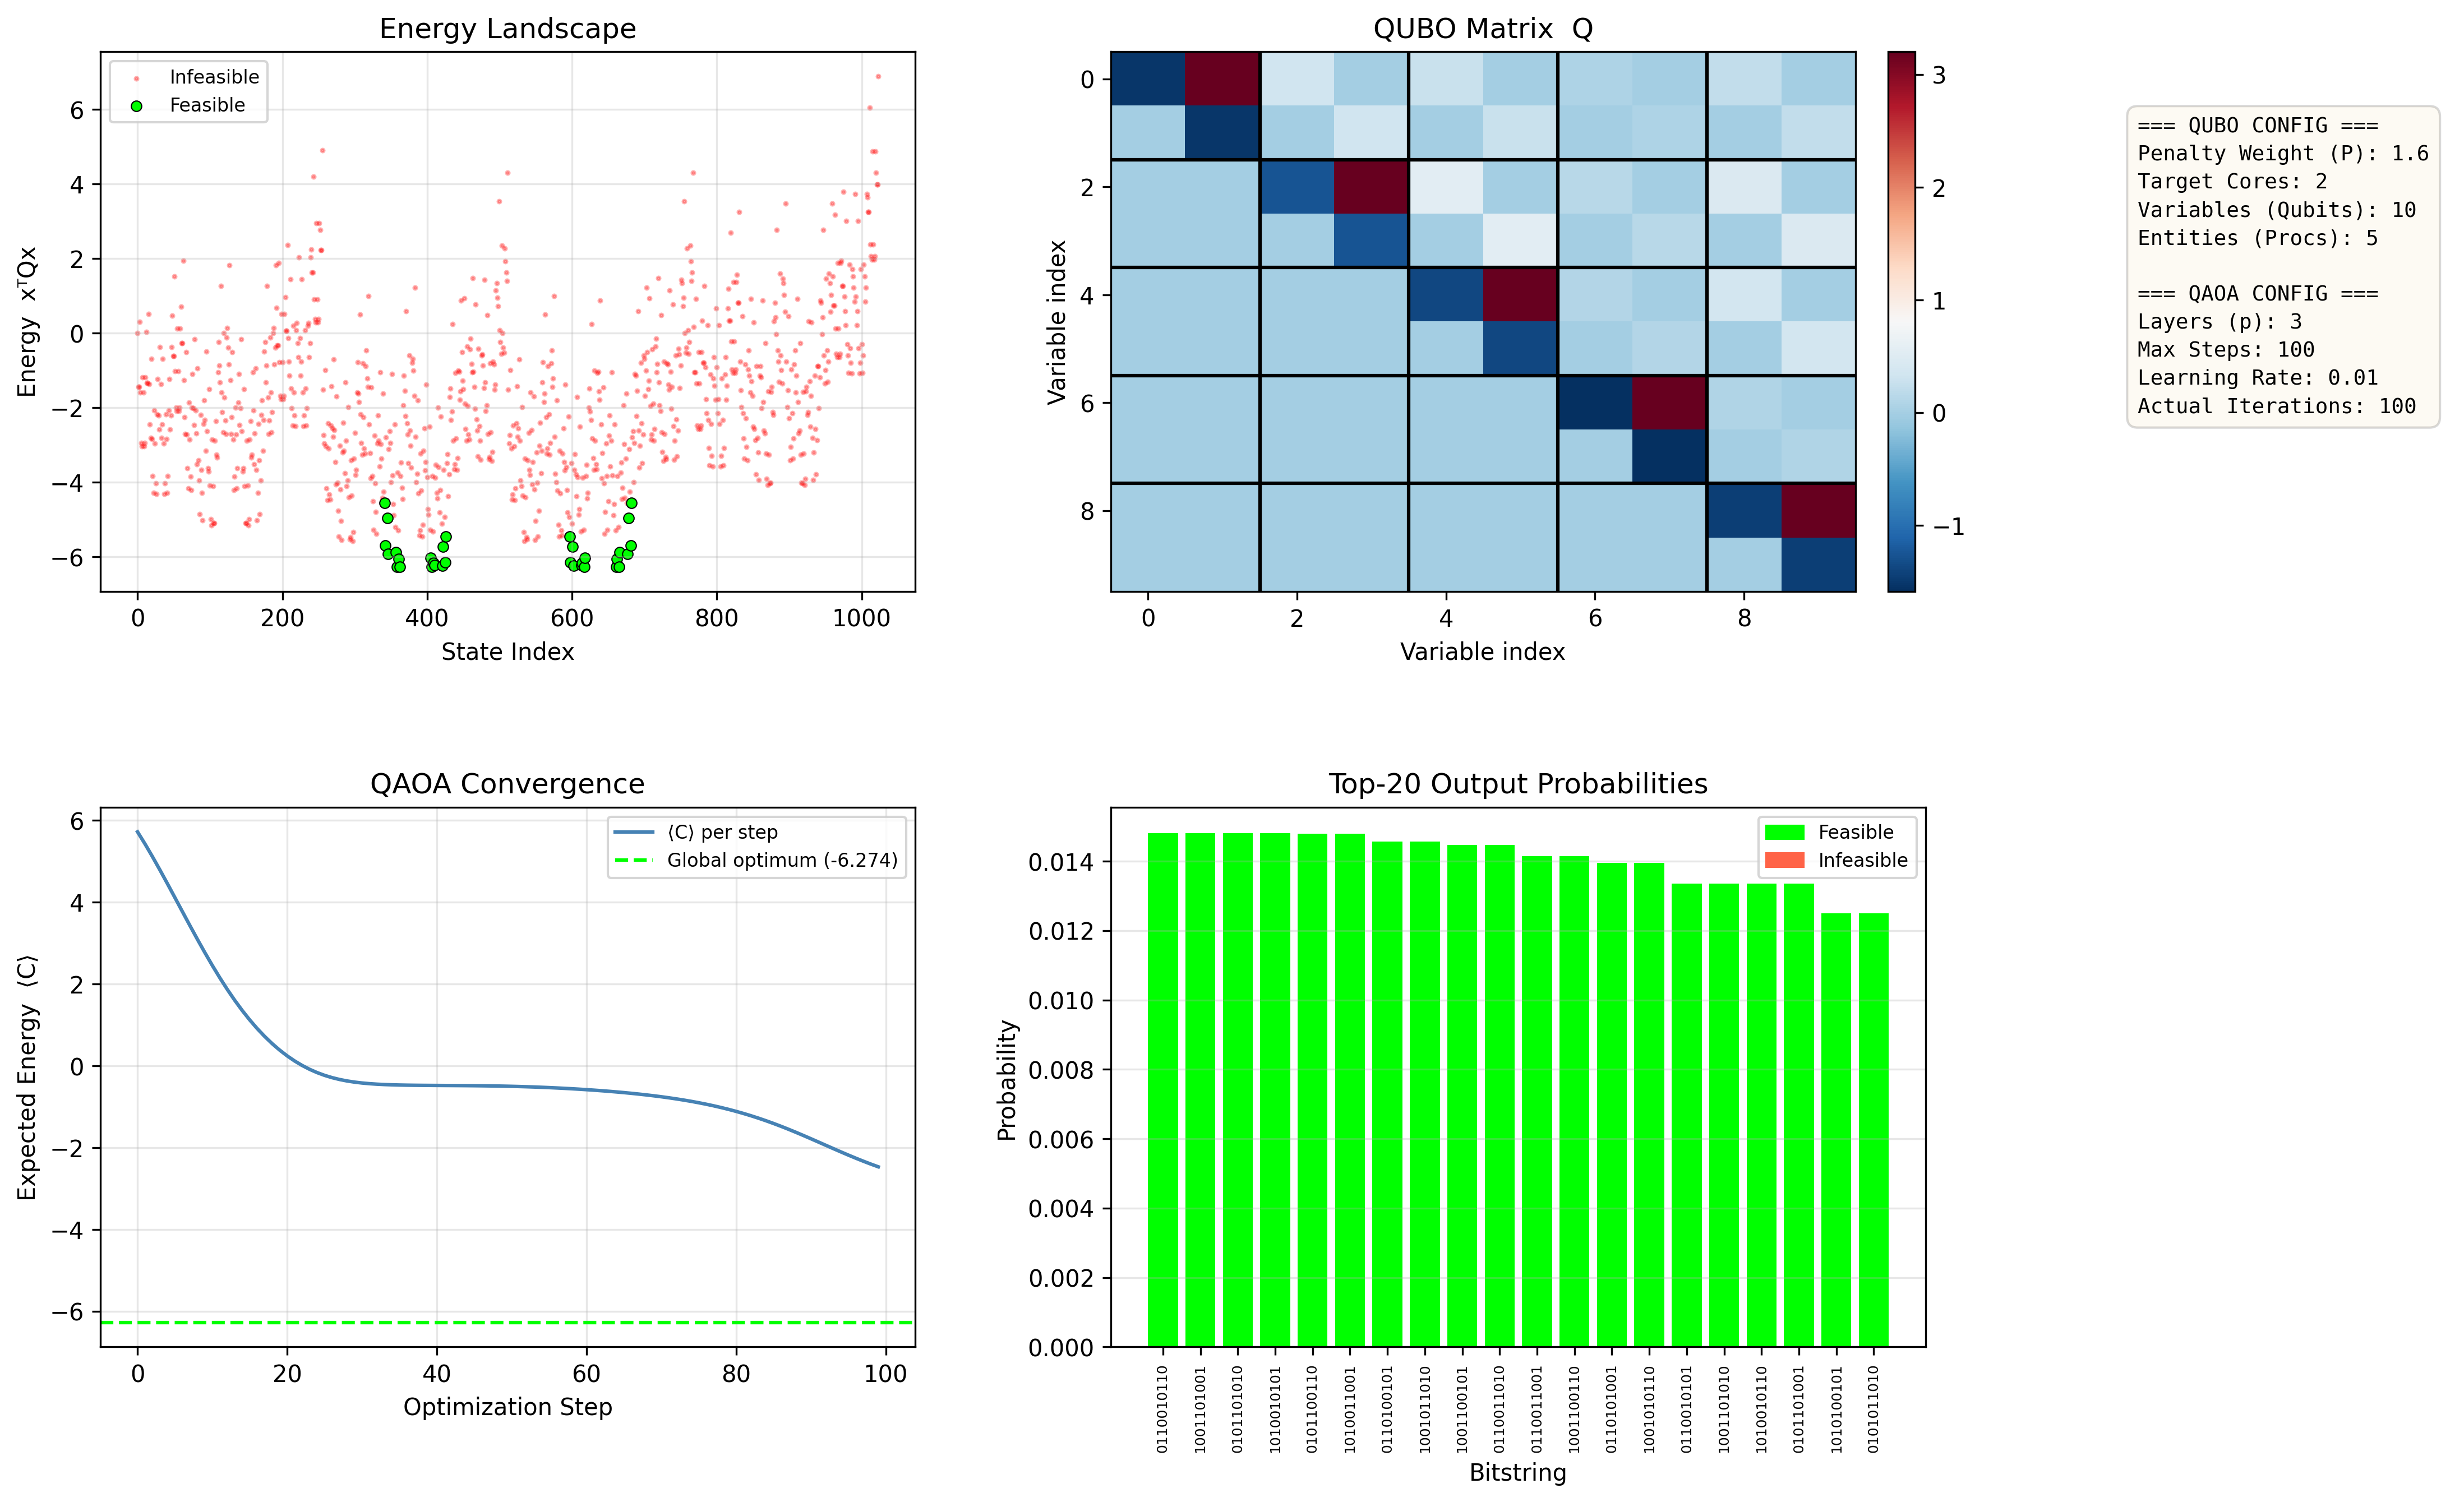
\includegraphics[width=0.9\textwidth]{../results/run_P1.6_p3.png}
  }{
    \fbox{\parbox{0.85\textwidth}{\centering
      \vspace{20mm}
      TODO: Add a default-pipeline visualization figure.
      \vspace{20mm}
    }}
  }
  \caption{Example direct QUBO/QAOA visualization.}
  \label{fig:direct-run}
\end{figure}

\chapter{Discussion}
\label{chap:discussion}

\section{Interpretation}

The prototype demonstrates that process-to-core assignment can be expressed as a
QUBO and connected to a hybrid optimization workflow. The strongest evidence is
obtained from small workloads where the brute-force oracle is available: QAOA
candidates can be checked for feasibility and compared against the exact
feasible optimum.

The iterative pipeline extends the experimental range by solving smaller
sub-QUBOs and propagating accumulated load between them. This gives the testbed
a practical way to study workloads beyond the direct simulation limit. However,
the iterative result is heuristic: each local decision may restrict later
choices, so global optimality is not guaranteed.

\section{Limitations}

The current work has several limitations:

\begin{itemize}
  \item The scheduling model only handles process-to-core assignment, not full
  preemptive time scheduling.
  \item CPU weights are snapshots rather than long-term workload predictions.
  \item The QAOA solver is simulated and therefore limited by classical memory
  and runtime.
  \item QAOA optimization is sensitive to initialization, depth, learning rate,
  and mixer choice.
  \item Live tracing depends on the state of the host machine during sampling.
  \item Brute-force validation is only available for small QUBOs.
  \item The XY-style mixer should be tested further before making strong claims
  about mixer superiority.
\end{itemize}

\section{Threats to Validity}

Internal validity may be affected by implementation bugs, stochastic optimizer
behavior, or incomplete experiment coverage. Construct validity may be affected
by the simplified scheduling objective, since real operating systems optimize
more than load balance. External validity is limited because the results are
obtained on simulated QAOA circuits rather than real quantum hardware and on a
limited set of workloads.

\chapter{Conclusion}
\label{chap:conclusion}

This thesis presented a hybrid quantum--classical testbed for studying a
simplified operating-system scheduling problem. The project formulates
process-to-core assignment as a QUBO, solves it with a PennyLane QAOA workflow,
validates small instances with brute force, and supports decomposition for
larger workloads. It also includes live process tracing, adaptive clustering,
visualization tools, a Streamlit interface, and a reproducible experiment
runner.

The prototype is best understood as an experimental platform. It provides the
infrastructure needed to compare QAOA behavior, validate feasibility, inspect
optimality gaps, and study decomposition strategies. The results so far are
promising for small and medium test cases, but the system remains a research
prototype rather than a production scheduler.

\section{Future Work}

Future work can extend the project in several directions:

\begin{itemize}
  \item Add stronger repeated-run statistics and parameter sweeps.
  \item Compare QAOA against classical heuristics such as greedy balancing,
  simulated annealing, and local search.
  \item Evaluate more realistic workload traces over time.
  \item Extend the model to include affinity, priority, migration cost, and
  deadlines.
  \item Improve sub-QUBO partitioning and investigate global repair steps after
  iterative assembly.
  \item Run selected QUBOs on real quantum hardware or managed quantum runtime
  services.
  \item Package result extraction into automatic LaTeX table generation.
\end{itemize}

\appendix

\chapter{Repository Map}

\begin{lstlisting}[caption={Project structure.}]
src/
  abstract/        Base interfaces
  builder/         QUBO builders
  decomposition/   Clustering, heuristics, sub-QUBO extraction
  pipeline/        Default and iterative scheduling flows
  solver/          QAOA, brute force, validation helpers
  tracer/          Live process snapshot collection
  visualizer/      Matplotlib and console visualizations
  experiments/     TOML scenarios and result runner
  app.py           Streamlit UI
  main.py          SchedulingEngine and CLI
  data_contracts.py
tests/
  test_builder_core.py
  test_brute_force_solver.py
\end{lstlisting}

\chapter{Key Configuration Objects}

\begin{lstlisting}[language=Python,caption={Representative configuration objects.}]
QAOAConfig(
    layers=1,
    steps=50,
    learning_rate=0.05,
    top_k=10,
    mixer_type="xy",
    init_gamma=0.5,
    init_beta=0.5,
)

QUBOConfig(
    penalty=5.0,
    num_cores=2,
    snapshot=None,
    target_load=None,
)

DecompositorConfig(
    qubit_max=8,
    num_cores=2,
    io_alpha=0.5,
    affinity_alpha=0.8,
    homogeneity_threshold=0.3,
    zscore_threshold=1.5,
    sorting_strategy=Heuristic.COUPLING_DESCENDING,
)
\end{lstlisting}

\chapter{Example Scenario File}

\begin{lstlisting}[caption={Example TOML scenario.}]
id = "T1.1"
tier = 1
category = "smoke"
name = "Minimal preset direct path"

[workload]
mode = "preset"
num_processes = 2
num_cores = 2
weights = [0.3, 0.7]

[qubo]
penalty = 5.0

[qaoa]
layers = 1
steps = 50
learning_rate = 0.05
top_k = 10
mixer_type = "xy"
init_gamma = 0.5
init_beta = 0.5

[decomposition]
qubit_max = 4
num_cores = 2
io_alpha = 0.5
affinity_alpha = 0.8
homogeneity_threshold = 0.3
zscore_threshold = 1.5
sorting_strategy = "COUPLING_DESCENDING"

[execution]
repeats = 1
\end{lstlisting}

\begin{thebibliography}{9}

\bibitem{farhi2014qaoa}
E. Farhi, J. Goldstone, and S. Gutmann,
\textit{A Quantum Approximate Optimization Algorithm},
arXiv preprint arXiv:1411.4028, 2014.

\bibitem{lucas2014ising}
A. Lucas,
\textit{Ising formulations of many NP problems},
Frontiers in Physics, vol. 2, 2014.

\bibitem{glover2018qubo}
F. Glover, G. Kochenberger, and Y. Du,
\textit{A Tutorial on Formulating and Using QUBO Models},
arXiv preprint arXiv:1811.11538, 2018.

\bibitem{pennylane}
V. Bergholm et al.,
\textit{PennyLane: Automatic differentiation of hybrid quantum-classical computations},
arXiv preprint arXiv:1811.04968, 2018.

\bibitem{silberschatz}
A. Silberschatz, P. B. Galvin, and G. Gagne,
\textit{Operating System Concepts},
Wiley.

\end{thebibliography}

\end{document}
